\documentclass[../main-v1.tex]{subfiles}
\begin{document}
\chapter{Workflow Management \hideme{McNab}}
\label{ch:wkflow}
%%%%%%%%%%%%%%%%%%%%%%%%%%%%%%%%
\section{Introduction}
\label{sec:flow:intro} 

The Workflow subsystem includes all aspects of orchestrating the execution of DUNE code to generate simulated data and to process real or simulated data at computing sites around the world. 

To make the most efficient use of the finite computing, network, and storage resources available to the experiment, the choices for the workflow system %anne 's choices 
are driven by the location and availability of data to be processed and it's %its 
 proximity to computing capacity as it becomes available to DUNE. Efficiently matching CPU and data is a long-standing problem in \dword{hep} computing. \dword{dune} proposes to use a relatively un-hierachical system that uses improved knowledge of the computing properties of applications (I/O rate, memory needs, data size) and the network connections between \dwords{rse} and \dwords{cpu} to optimally match processing and data. 

This chapter describes the existing production system which is being used to process data from \dword{protodune}, and %then 
explains the requirements for the future system and the prototype of it that has been produced. %anne  which has been produced of it.

% The Workflow subsystem caches information provided by the Data 
% Management and Information subsystems and uses it to make its
% decisions.


\section{Existing Production Submission Infrastructure \hideme{Herner - draft}}
\label{sec:current}

\subsection{Production Operations Management System}
\label{subsec:jobsub}

Production and large-scale analysis jobs currently use \dword{fnal}'s \dword{poms}~\cite{Mengel:2020wev} for submission. \dword{poms} provides both GUI and command-line options for job launches (both immediate and scheduled), recovery project setup, and provides integrated monitoring with \dword{fnal}'s Landscape project. Job submission is typically via \dword{fnal}'s \dword{jobsub} tool~\cite{box2014fife}. \dword{jobsub} in
turn interfaces with the \dword{glideinwms} workflow management system~\cite{sfiligoi2009pilot} for resource provisioning and matchmaking to slots at \dword{fnal}, on dedicated DUNE resources at other sites, or opportunistic cycles on the \dword{osg}   and \dword{wlcg}. Figure~\ref{fig:workflowPOMS} illustrates the entire chain, including interaction with storage elements within the job.
The architecture can also provision resources on \dword{hpc} resources, such as Cori at the \dword{nersc}, within the HEPCloud~\cite{mhashilkar2019hepcloud} infrastructure. The submission mechanism is unchanged whether the jobs are \dword{htc} or \dword{hpc}; this seamless transition is key to efficiently utilizing available resources and also saves the job submitter significant effort by not requiring customized submission infrastructure for different resource types.

\begin{figure*}[htb]
\centering
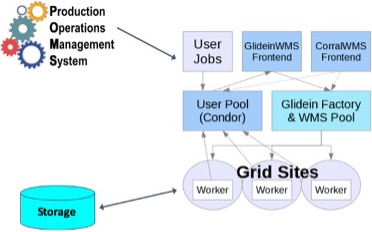
\includegraphics[width=.7\textwidth]{graphics/Workflow/POMSWorkflow.jpg}
\caption{Overview of the current DUNE Production workflow setup used also by the \dword{protodune} detectors for data reconstruction and simulation. Production group members interact with \dword{poms} to submit jobs, which uses the \dword{jobsub} tool to submit jobs to a HTCondor scheduler. \dword{glideinwms} provisions worker node resources and jobs match to the available worker node slots. DUNE jobs interact with storage elements  at \dword{fnal} and other sites both for input copy (or streaming for most production workflows) and output copyback.}
\label{fig:workflowPOMS}       % Give a unique label
\end{figure*}

Choosing a Glidein-based system at this stage of the experiment had several advantages. DUNE was able to quickly leverage the existing FIFE~\cite{herner2019advances} toolset, including \dword{poms} and \dword{jobsub}, negating the
need for significant effort from the experiment in getting jobs running quickly (let alone in designing a completely new system). Since the system is in use by other neutrino experiments at \dword{fnal}, it is easy for new DUNE collaboration members coming from these experiments to 
begin submitting jobs quickly as they are working with a familiar system. The DUNE production workflows were also able to leverage the existing infrastructure support teams in place to serve other collaborations and consortia such as 
CMS and \dword{osg}. Finally, as \dword{glideinwms} is widely used in HEP, setting up new sites becomes extremely straightforward, especially if the site is already supporting another experiment that uses \dword{glideinwms}. Our integration times for new 
DUNE sites are typically less than one week and successful production jobs immediately after opening up the site are now the rule rather than the exception. This ease of setup has been a key enabler of DUNE's international expansion. International sites routinely deliver more than 50\% of \dword{dune}'s \dword{cpu} resources as illustrated by  the total DUNE Production wall hours for August 2021  shown in Figure~\ref{fig-country}. International sites regularly run the full suite of DUNE jobs, including \dword{protodune} data reconstruction and user analysis. % DUNE is also considering the creation of a global GlideinWMS pool similar to the CMS Global Pool~\cite{cmsgp,cmsgp2}, which would enable multiple institutions to set up their own submission hosts if they desired to do so.

\begin{figure*}[htb]
\centering
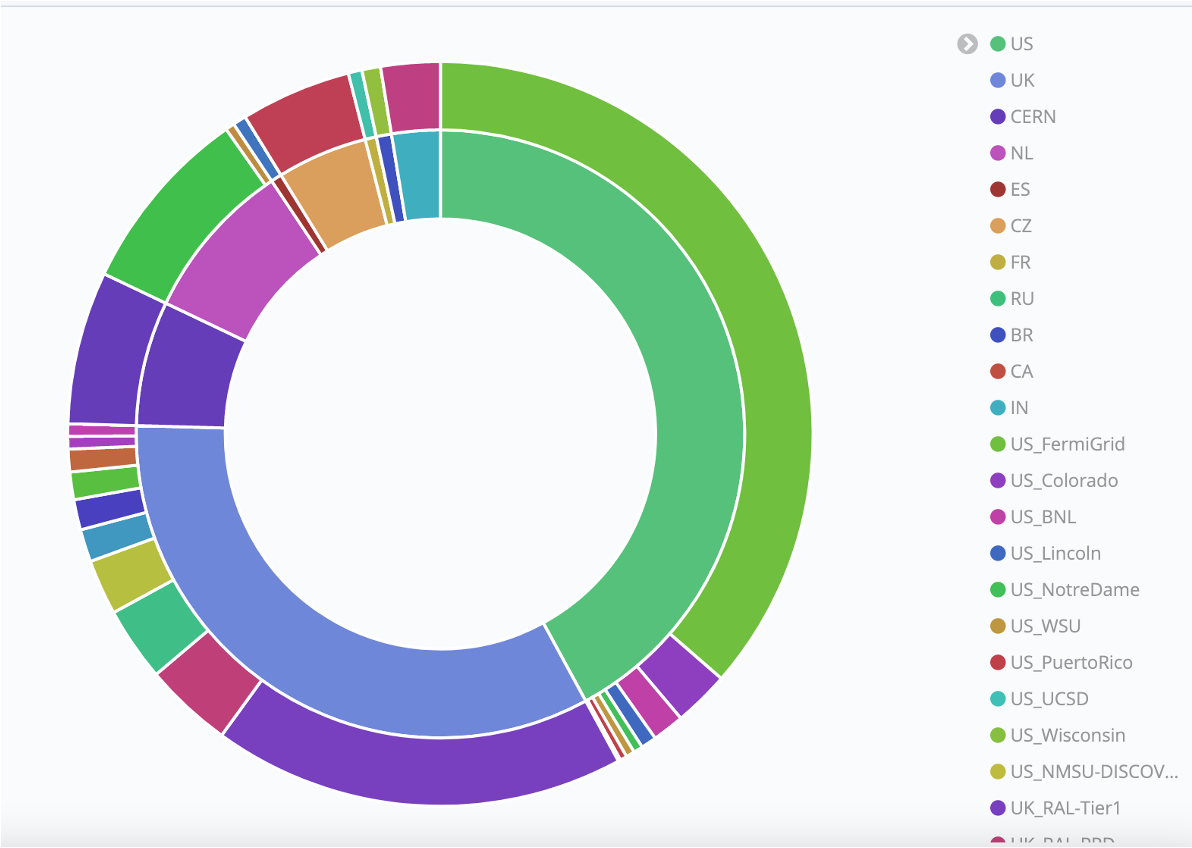
\includegraphics[width=.8\textwidth]{graphics/Workflow/August2021.png}
\caption{Wall time-weighted distribution of successful DUNE Production jobs for August 2021. Inner ring: distribution by country. Outer ring: distribution by site. Sites outside the U.S. delivered 60\%\ of the total wall hours for the jobs shown here.}
\label{fig-country}       % Give a unique label
\end{figure*}

\subsection{%DUNE 
Software, Input Data Distribution, and Output File Handling}
\label{subsec:io}
DUNE builds its software suite for  Scientific Linux. Since October 2019 DUNE jobs %will 
have been automatically run inside a Singularity container at supported sites via a \dword{glideinwms} mechanism that requires no user knowledge of Singularity other than specifying the desired image. This %reducing the possibility of errors and guaranteeing a 
reduces the possibility of errors and guarantees ahomogeneous environment across all sites.

For its file catalog, DUNE uses \dword{fnal}'s \dword{sam} system~\cite{Illingworth:2014mba}, which handles input file selection and delivery for each job, and has been successfully used by numerous HEP experiments for well over a decade. As described in Chapter \ref{ch:datamgmt},  in future we expect \dword{rucio}~\cite{Barisits:2019fyl} will  take over most of these functions. Production jobs typically stream input data files via \dword{xrootd}, though in some cases they will copy a file to the worker node and directly read the local copy. The data source can be any storage system reachable from the worker
node and to which DUNE has access. This is frequently \dword{fnal} \dword{dcache}, but \dword{eos} at the \dword{cern} and other storage elements in Europe are also used (jobs run at \dword{cern} would get their inputs from \dword{cern} \dword{eos}, for example). 

We have recently implemented minimal match optimization between \dwords{rse} and compute sites in \dword{sam} as many data samples used for user analysis have now been duplicated at European \dwords{rse}.  \dword{sam} now directs data from European sites to jobs running in Europe when possible.  This is done via a reasonably simple look-up table that provides a prioritized list of data locations for each compute site.  Even this simple system substantially raised the efficiency for high IO applications at many sites. Section \ref{ch:model:perf} describes studies of rse-to-cpu data rates that were used to implement the priority tables. 



Several DUNE workflows require one or more auxiliary input files %not needed (i.e. not detector data) 
such as calibration files or neutrino flux information, and other inputs necessary for analysis for \dword{mc} generation. Some simulation workflows randomly
choose several such input files for each job from a much larger set, so the file overlap between jobs is small. Additionally the files are typically tens of MB in size. These two attributes make these files poor candidates for placement in a standard \dword{cvmfs} repository. For such files we store them in a \dword{stashcache}~\cite{bib:stashcache} repository,
accessible in a POSIX-like fashion though a \dword{cvmfs} overlay. With this method there is still some level of shared caching on a worker node, but as files need to be copied in from the source (\dword{fnal} \dword{dcache}), it happens in a transparent way, meaning the user can simply access the files via a \dword{cvmfs} path in the {\tt dune.osgstorage.org} repository.

For output file handling nearly all workflows currently copy their outputs to \dword{fnal} \dword{dcache}, with a small minority (\dword{pddp} jobs) also copying to a storage element at IN2P3 in France. We use \dword{rucio} to manage file replication
to other sites. In the future DUNE will likely move to a more distributed copyback model: at sites with local storage, a job can simply copy its output to a local location, and then we can use \dword{rucio} for replication as is already done, rather than requiring everything first go through \dword{fnal}.

There is an exception for workflows run at NERSC; we read input auxiliary files from and copy output files out
to Cori's global scratch filesystem. For job outputs, a separate process performs bulk transfer back to \dword{fnal} from one of \dword{nersc}'s dedicated data transfer nodes. We expect that workflows on other future \dword{hpc} platforms
will follow a similar approach, especially at places without external connectivity on the worker nodes.

\section{Requirements for Replacing SAM Functionality}

As well as the data management functionality of \dword{sam} described earlier, it will be necessary to provide a replacement for \dword{sam}'s role in assigning work to jobs and keeping track of what work has been done. We propose to take this opportunity to extend the \dword{sam} model further, by allowing the replacement system to determine which requests for work should be processed at a particular place and time, as well as determining which file to process next.

% this next paragraph should be founded on stuff in the computing
% model chapters' description of what kinds of resources there are
Discussions with partner projects reveal a variety of constraints imposed by the circumstances of different sites. Some sites have 
abundant network capacity and can readily support jobs that stream input data from elsewhere. Others have relatively limited networking
compared to the volume of computing power they make available, and
expect experiments to only send jobs that will process %the data they
stored onsite. A third class of sites has access to metropolitan or 
regional networks that can accommodate streaming from nearby sites only.
%anne but not from elsewhere.

This landscape has led us to look at %anne models where 
systems in which jobs can be matched to sites where their input data is present, to deal with the most constrained class of sites. %anne, but which 
However, the system must allow us to be progressively more relaxed about data access for jobs running at %other 
less constrained sites. %anne depending on their situation and on how heavily that type of job uses input data.
 

%A further constraint is the 
Further, the system will need to evolve the large user code base and ways of working that are currently based on \dword{sam}. For example, the %existing applications assume that \dword{sam} will supply the name and location of the next file to be processed when queried by jobs which are tied to a particular \dword{sam} project and its dataset. 
existing applications assume that, when queried by jobs that are tied to a particular \dword{sam} project and its dataset, \dword{sam} will supply the name and location of the next file to be processed. 

To accommodate %anne both sets of 
these constraints, we have designed and prototyped a generalization of the \dword{sam} model. Using our Sites and Services model described in Section~\ref{sec:cm:sites_and_services}, generic jobs arrive at grid worker nodes on a Computing Element at a site and ask a central Workflow Allocator what they are to work on and which file to process within that activity. This matching is based on the physical characteristics of the worker node job slot (such as memory, processors, and lifetime) and what data are unprocessed and suitable to be accessed from local or remote Storage Elements. 


\section{Request Lifecycle}
\label{sec:flow:lifecycle}

The central concept of the proposed workflow system is a request %, which 
that describes how some data processing activity is to be carried out. Requests are submitted by users (which may include members of a central production team) to the Workflow Database described below, where it progresses through %anne. Each request can be in one of 
several states, %anne, which it progresses through. 
for example, draft > submitted > approved > running > paused > running > checking > completed > archived. Human intervention is needed for some transitions, e.g., from submitted to approved. Requests also have types and priorities. For example, simulation or user analysis, and high or low, respectively.

As part of its definition, a request may include one or more stages, each of which can apply a sequence of processing steps to the input or output files. %anne the request uses or generates. 
%anne Each stage specifies a bootstrap script used by generic jobs to run the relevant applications, requirements on the worker nodes eligible to run that stage (for example memory), and the maximum number of input files to be issued to a generic job executing that stage.
Each stage specifies a bootstrap script used by generic jobs to run the relevant applications. The script specifies the requirements on the worker nodes %anne eligible to run that stage 
(for example memory) and the maximum number of input files to be issued to %a generic 
the job executing that stage.

The %definition of a 
request definition will include an \dword{metacat} MQL query % not needed which can be submitted to \dword{metacat} 
to generate a list of files to be processed in the first stage. This list of files is cached in the central Workflow Database, associated with the first stage of that request. All these files are set to the unallocated state. 

The request definition is an input to the Data Management placement agent, which transfers replicas of files to suitable sites as necessary. %(anne)not necessary based on the description of the request and knowledge of site features. 
The location of the replicas of the files is also included in the database, cached from \dword{rucio}. 

Once the various agents have finished building the request, it can move to the running state and the bootstrap script associated with the first stage will begin execution. %(anne)not necessary to be executed at sites to process files.


\begin{dunefigure}
[Workflow and data management architecture diagram]
{fig:workflow} 
{Workflow and data management architecture diagram.}
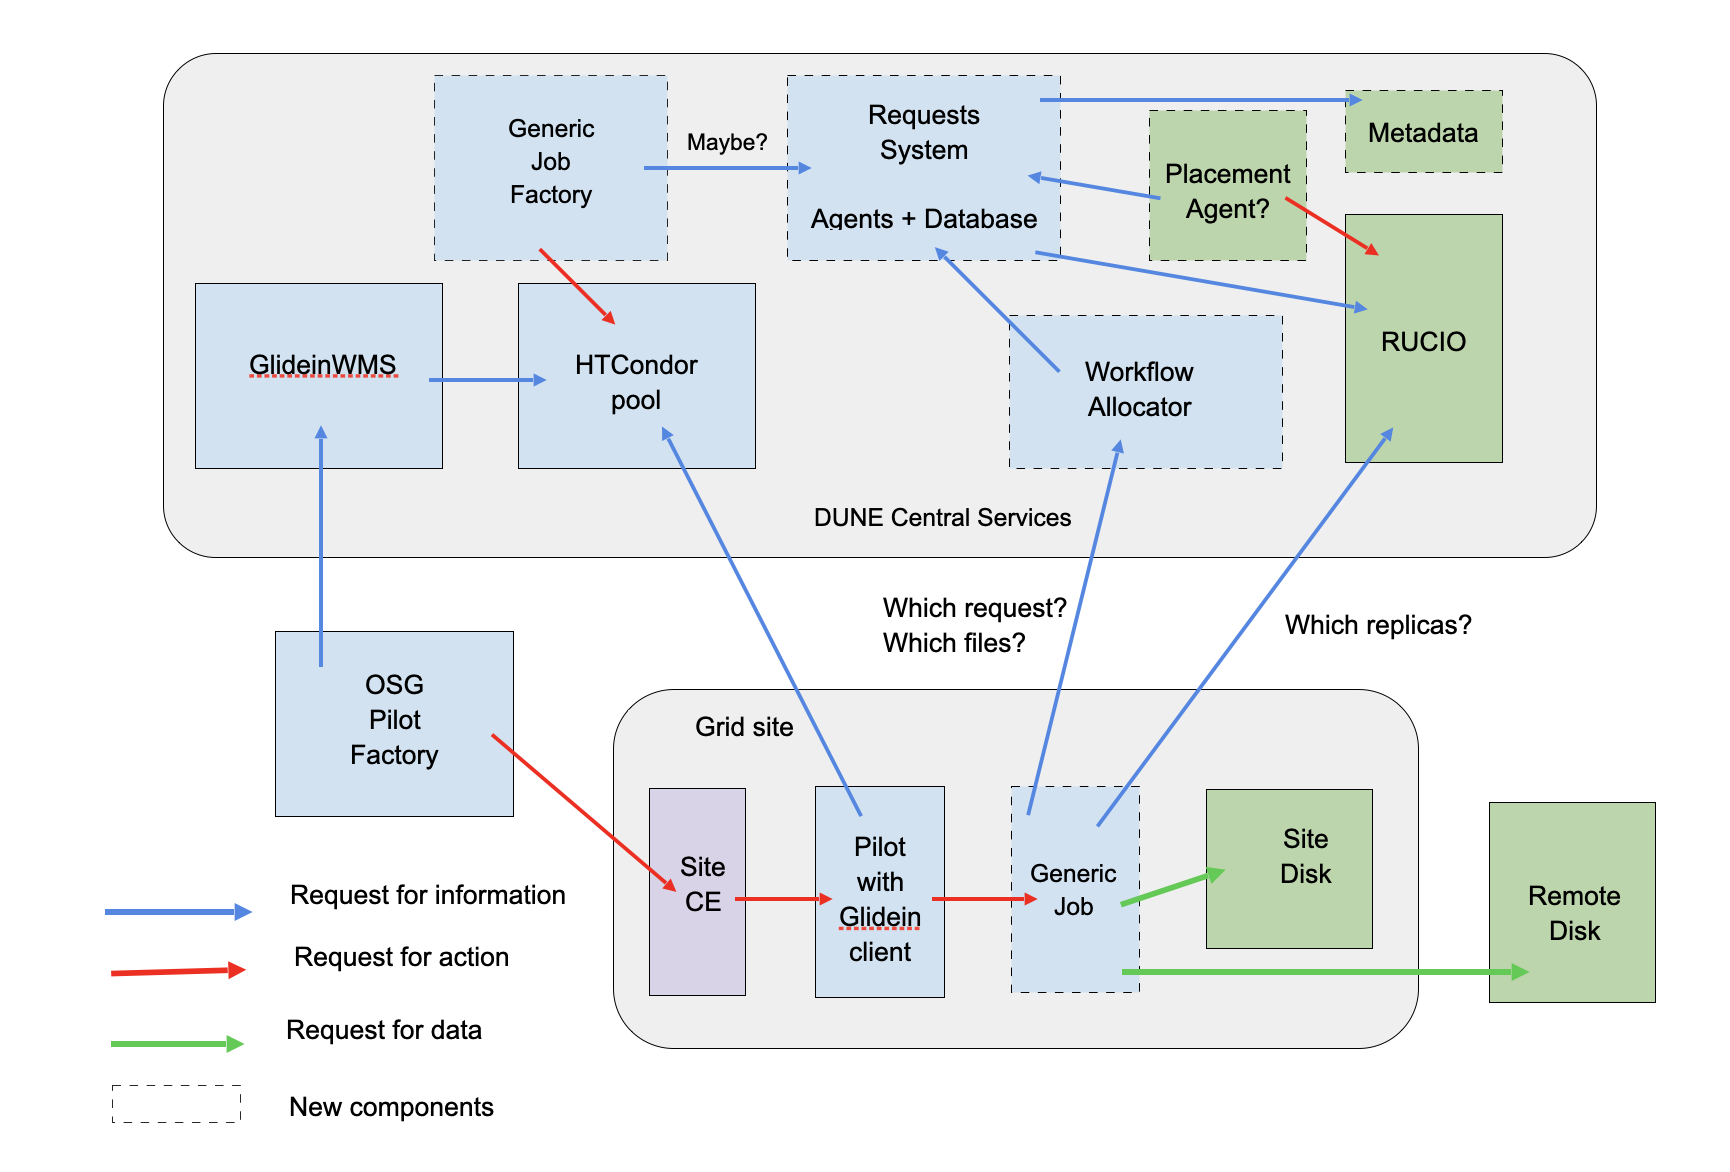
\includegraphics[height=8cm]{graphics/Workflow/wfs.png}
\end{dunefigure}

\section{Grid Workload Systems}
\label{sec:flow:grid}

The workflow system makes use of the existing global grid infrastructures to deliver jobs for execution on worker nodes at sites. This allows us to operate alongside other experiments in the \dword{wlcg} without placing special requirements on sites.

\dword{fnal} operates a global HTCondor pool for DUNE which makes use of the existing \dword{osg} Pilot Factory service and HEPCloud to provision execution slots at sites. By using these existing systems we are able to use computing capacity presented with ARC CE or HTCondor CE grid interfaces, or on cloud and \dword{htc} services supported by HEPCloud.

\section{Generic Job Factory}
\label{sec:flow:factory}

The Generic Job Factory agent creates and submits HTCondor jobs, which are each assigned to a specific execution site. It will use a mixture of matching successes, site limits from DUNE \dword{cric}, and prioritization of sites to determine how many generic jobs to submit and have waiting at each site. It may also use inspection of the central workflow database to estimate whether more generic jobs should be submitted for a particular site. For ordinary jobs, the job factory must be able to prioritize use of pledged academic and lab sites over commercial cloud sites and specialized sites like \dword{nersc}, which are managed by HEPCloud, to allow those services to be used for specialized workflows. Inspection of files waiting to be allocated in the database may be more appropriate for HEPCloud managed sites, so that work requiring their features may be satisfied.

Once a generic job lands on a worker node, it contacts the Workflow Allocator described later which determines which unallocated files from one stage best match that worker node.

\section{Workflow Database}
\label{sec:flow:wfdb}

The central Workflow Database stores definitions of requests and their stages, and cached information about files, replicas, sites, and storage services. Together all this information is used by queries to determine what work to carry out where. It is implemented as an SQL relational database.

\section{Information Collector}
\label{sec:flow:collector}

The Information Collector agent runs periodically to obtain a list of eligible sites and storage services from \dword{cric} and other information sources, including any downtime notifications. This information includes a table recording whether data access from a particular site to a particular storage is classed as being at the same site, a ``nearby'' site, or is merely elsewhere on the grid but not blocked by firewalls or policies (for example at an \dword{hpc} site with no off site access.) The concept of ``nearby'' is defined as being accessible with an acceptable level of inefficiency.

\section{Request Builder}
\label{sec:flow:builder}

The Request Builder agent uses the input dataset definition in a request to construct a list of input files for the first stage of that request. Typically this involves making queries to MetaCat to obtain a list of files in the given dataset. This list is cached within the Workflow Database so it can be used as part of SQL queries. As the files are identified, the location of their replicas are also obtained and cached from RUCIO. Again, this allows the proximity of replicas of unprocessed files to be used in deciding what work a job should do.

\section{Archiver}
\label{sec:flow:archiver}

The Archiver agent has responsibility for removing information about requests, stage, files, and replicas once they are no longer needed, archiving whatever is needed for future reference to long term storage. It is intended that important information about how and where files were processed will be stored in the MetaCat database by the generic jobs themselves, but some higher level information about the operation of the workflow system and the processing of requests will be saved by the Archiver.

\section{Workflow Allocator}
\label{sec:flow:allocator}

Once a generic job arrives at a worker node, it contacts the Workflow Allocator service which determines which unallocated file from one stage best matches that worker node. This matching includes the characteristics of the worker node job slot (memory, time limit etc), and whether the site is eligible to access a replica of that data file. The matching takes into account that some stage definitions allow access to remote input files anywhere on the grid, and others require files to be at a ``nearby'' site. Replicas are prioritised based on whether the worker node and replica are at the same site, ``nearby'', or elsewhere but still eligible. 

The bootstrap script to run and details of the request and stage are returned to the generic job. The script can use these details to request a series of files to process with the application it invokes. Each input file successfully processed by the application is reported to the Workflow Allocator so that the input file’s status can be updated from Allocated to Processed. Unprocessed input files are returned to the unallocated state for processing in another job. 

If the stage is not the final stage for that request, each output data file is also inserted into the list of files associated with the next stage for that request, in the unallocated state. 

\section{User Commands}
\label{sec:flow:commands}

Command line tools are provided to operators and users to allow queries of Workflow Database contents and the creation of requests. These tools are envisaged to be of most use during testing of new workflows and for short workflows during analysis. 

\section{Workflow Dashboard}
\label{sec:flow:dashboard}

The same functionality as the command line tools outlined above is provided by a Workflow Dashboard web interface. This will allow more sophisticated searches in the Workflow Database to monitor the progress of running requests, and allow members of the operations team to examine the state of the system at the level of individual files and replicas which are due to be processed, or have recently been processed to enable debugging of problems with sites or workflow definitions.

The Workflow Dashboard is also intended to be used for all large scale productions, and will allow submitters to draft request definitions, circulate their proposal with colleagues for checking, before submitting them to any formal approval and checking procedure. The lifecycle of a workflow request accommodates manual approval and prioritization of large requests while smaller requests can be approved automatically according to a preset limits. A library of bootstrap script templates and requests will be provided as part of the dashboard to help users make sensible choices for common types of workflow.

\section{Workflow System Prototype}
\label{sec:flow:prototype}

A prototype implementation has been produced, which includes the Workflow Database, Workflow Allocator service, command line tool, generic job script, and the monitoring aspects of the Workflow Dashboard. Tasks to be carried out asychronously by the various agents are currently done with ad-hoc scripts, which are gradually being replaced by agents.

Using this prototype, we have created requests based on existing productions, populated them with lists of files and replicas held by RUCIO, and then processed the files within generic jobs executing the bootstrap script included in the stage definitions, as sites, using matching perfomed by the Workflow Allocator.

\section{Implementation Plan \hideme{McNab/Timm/Herner needed}}
\label{sec:flow:implementation}

During 2022, We plan to continue increasing the number of components of the design implemented in the prototype until it becomes a viable system which can be used for production processing of protoDUNE data. This will allow further comparisons between the functionality requirements of the production team and users, and the Workflow System design.

% How much more to say about this?

\end{document}